\paragraph{Задание}

Спроектировать базу данных и создать приложение для автоматизации работы фирмы по производству обуви.
База данных должна хранить данные о каждом сотруднике, список поставщиков необходимой продукции или комплектующих и данные о каждом поставщике, список поставляемой продукции или комплектующих, список выполняемых сотрудниками работ.
Каждый поставщик может поставлять несколько видов продукции.
Каждый сотрудник может выполнять несколько видов работ, каждый вид работ может выполняться несколькими сотрудниками.

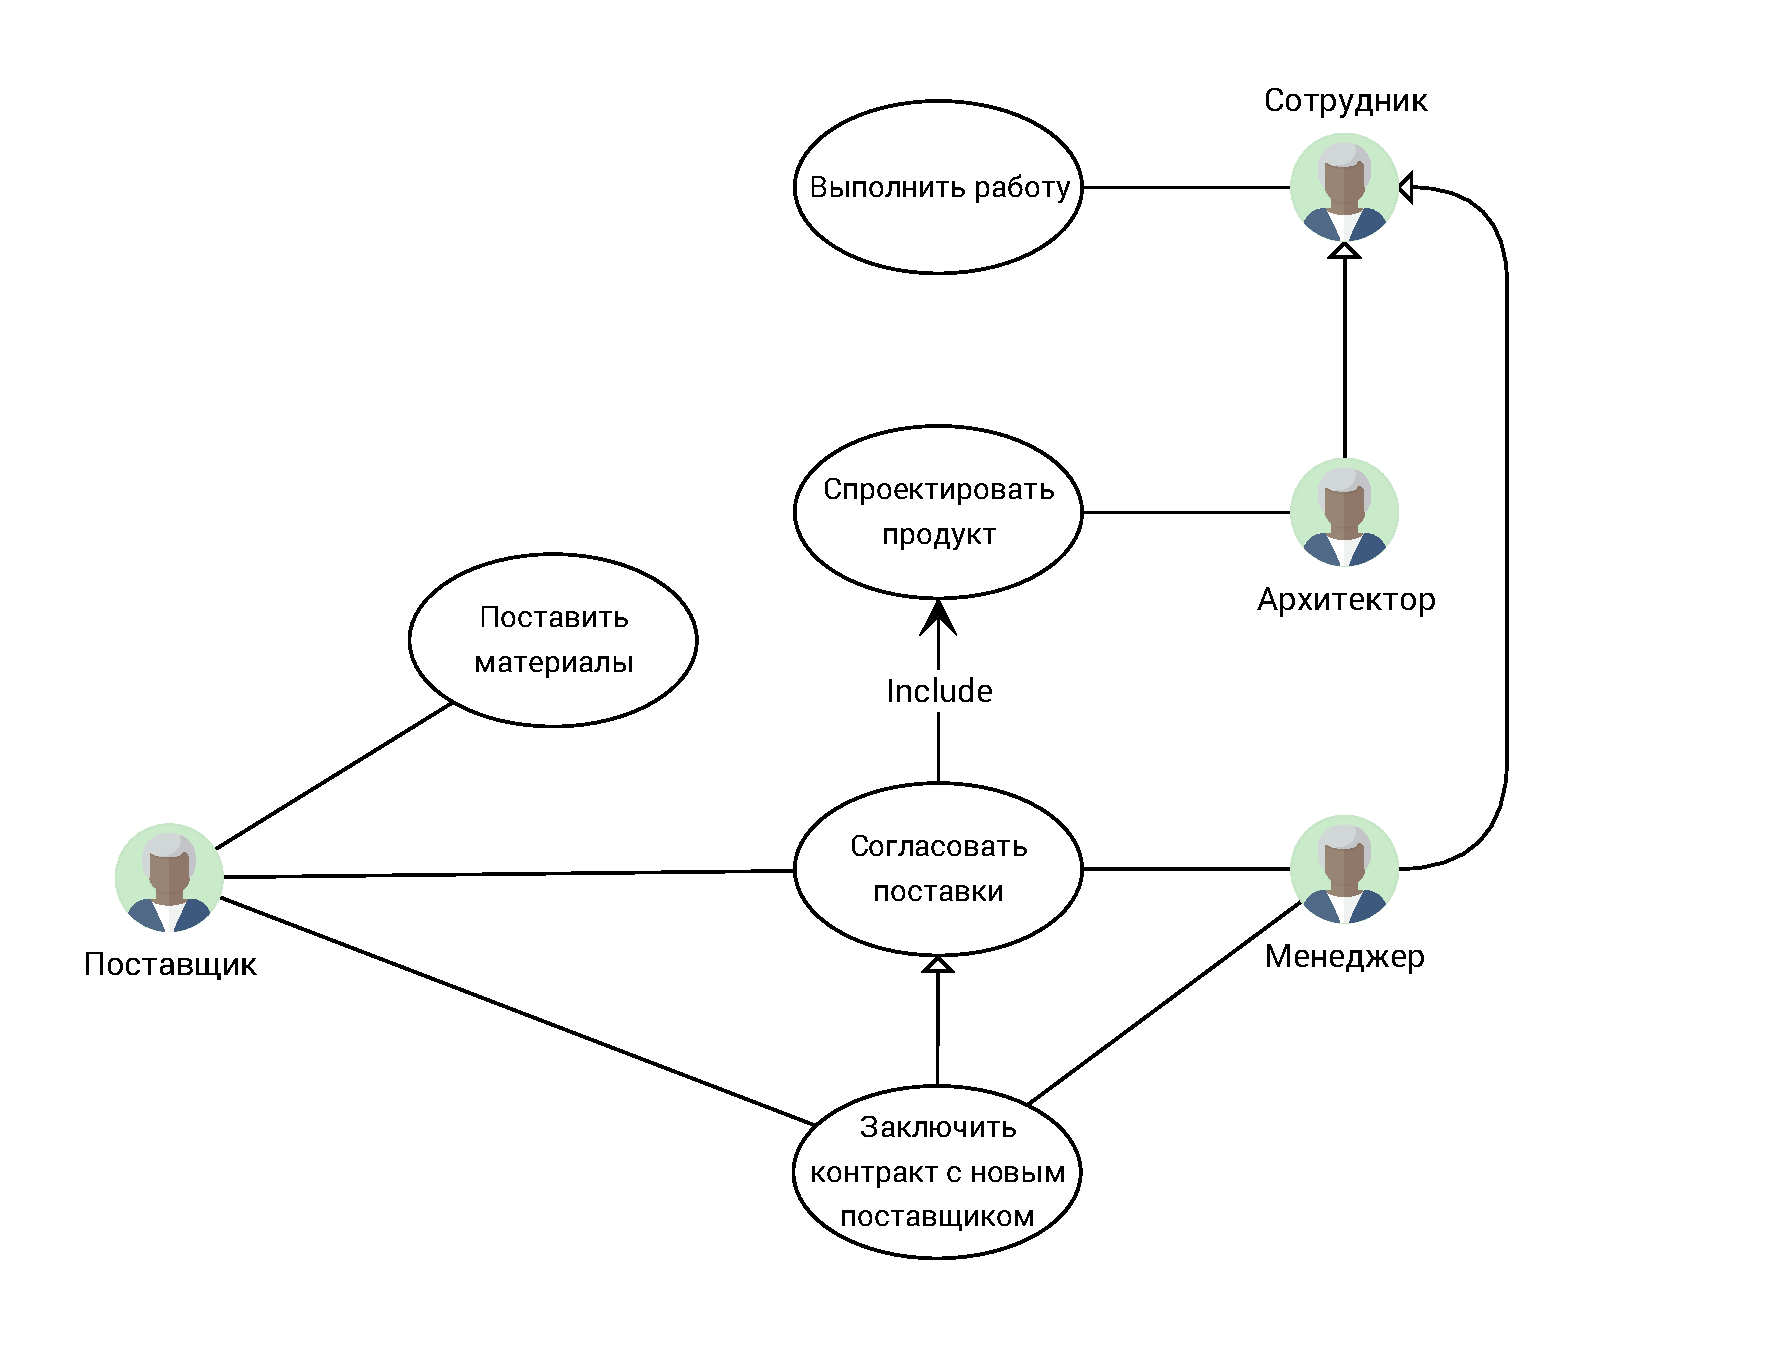
\includegraphics[width=0.9\textwidth]{social-network.pdf}

% Please add the following required packages to your document preamble:
% \usepackage{multirow}
\begin{table}[]
    \begin{tabular}{|l|l|l|l|}
        \hline
        Актёр                      & Цель                                  & Успех                  & Исключение       \\ \hline
        Сотрудник                  & Выполнить работу                      & Успех                  &                  \\ \hline
        Архитектор                 & Спроектировать проект                 & Успех                  &                  \\ \hline
        \multirow{3}{*}{Менеджер}  & \multirow{2}{*}{Согласовать поставки} & \multirow{2}{*}{Успех} & Проект не создан \\ \cline{4-4}
                                   &                                       &                        & Нет поставщиков  \\ \cline{2-4}
                                   & Заключить контракт с поставщиком      & Успех                  &                  \\ \hline
        \multirow{3}{*}{Поставщик} & Поставить материалы                   & Успех                  & Нет материалов   \\ \cline{2-4}
                                   & Договориться о поставках              & Успех                  & Нет материалов   \\ \cline{2-4}
                                   & Заключить контракт                    & Успех                  &                  \\ \hline
    \end{tabular}
\end{table}